\chapter{Literature Review}\label{c:literature}

\section{What is a Literature Review}
Literature Research is also referred to as Literature Study or Literature Review.
It is individual work on a topic agreed upon between the thesis supervisor and the student.
It involves creating a research question that can be answered using the existing literature, finding and analyzing the right literature, and writing a solid report about it.

% FROM HRI MANUAL
This chapter aims to give guidelines and suggestions to help you in writing your literature report. Typically the report writing takes three months and can roughly be divided into three phases, each requiring approximately one month’s work:
\begin{enumerate}
    \item Orientation \& exploration.
    \item Structured literature search.
    \item Literature documentation.
\end{enumerate}

\begin{figure}[h!]
	\centering
	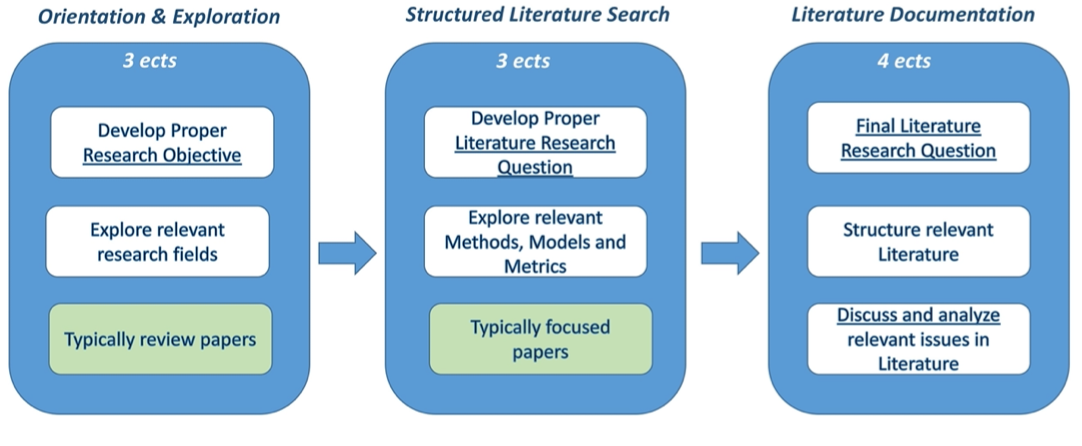
\includegraphics[width=0.8\textwidth]{figures/literatu_study_process.png}
	\caption{Overview of the literature study, reproduced from \cite{Master Thesis Guide, HRI section Cognitive Robotics}.}
	\label{fig:dexnet3_functionality}
\end{figure}

\section{Literature Review in the MSc Robotics program}
The Literature Review is called the Literature Research in the MSc Robotics Program, and it is 10EC
In detail, from the Study Guide \url{https://studiegids.tudelft.nl/}:

\begin{quote}
The aim of the literature study is to learn how to independently search for recent scientific publications (i.e., articles, theses, books). The literature study is carried out individually. The topic of the literature study is linked to the graduation project. The findings from the literature study are used to motivate the research plan of the thesis and are instrumental for achieving a high-quality final thesis.
\end{quote}

Learning Objectives:
After completing their literature research, students will be able to:
\begin{itemize}
    \item study a topic by critically selecting relevant scientific literature,
    \item identify and acquire lacking expertise
    \item identify the most interesting and relevant questions or problems in the field of the MSc thesis
    \item analyse and solve engineering problems in a systematic way
    \item present and report in good English
\end{itemize}

This part of your graduation process includes the following activities which are assessed:
\begin{itemize}
    \item Literature Research (written report; minimum grade: 6.0). The report is graded by the supervisor.
    \item Presentation (colloquium) (pass/fail). The presentation is combined with the introductory phase of the MSc project. The colloquium is graded by an ad-hoc committee of scientific employees of the department.
    \item Colloquium Attendance (pass/fail). All students must attend at least 10 colloquia.
\end{itemize}
	
\section{Literature Review at KAS Lab}
